%%This is a very basic article template.
%%There is just one section and two subsections.
\documentclass[twocolumn]{article}
\usepackage{graphicx}
\usepackage{amsmath}
\usepackage{amssymb}
\usepackage{subfigure}
\usepackage{epstopdf}
\epstopdfsetup{update} % only regenerate pdf files when eps file is newer
\title{Tuning plasmon of gold nanorods by KCN etching}
\author{Aquiles Carattino \and Pedro Navarro \and Saumya Khatua \and Michel
Orrit}

\begin{document}
\maketitle
\abstract{This is the abstract}

\section{Introduction}
Gold nanoparticles exhibit a collective oscillation of conduction electrons
known as the plasmon resonance of the particle. This resonance depends on the
aspect ratio (AR) of the particle and can be found from  $540\,nm$ for spheres
(AR of $1$) to even above $1500\,nm$ for nanorods (AuNR). This makes the gold
nanoparticles particularly suitable for a range of experiments, and applications
extending from solar cells production\cite{catchpoleplasmonic2008} to biosensing
and photodynamic therapy.

Tuning the resonance of the particles is useful when there is the need of having
control over the spectral properties of these structures. For instance it may be
needed to have a particle with a resonance coinciding with the available lasers;
or it may be needed to have control over the spectral response for generating
narrow transparency windows\cite{biswasplasmon-induced2013}.

Usually the tuning of the resonance is done at the moment of the synthesis. By
controlling the concentrations of growth and seed solutions it is possible to
induce the formation of longer or shorter particles. This methods, however,
always present a big dispertion in their outcome. This hinders the repeteability
and the ability to build larger, repetitive structures.

It is therefore useful a method that allows the in-situ control of the plasmon
resonance. This work shows that is possible to change the plasmon resonance in
more than $100\,nm$ without degrading the optical properties (i.e. the FWHM of
the peak.) For doing so it is employed KCN as an etching agent; a known and well
understood compound that is used not only in the nano-industry but also at
bigger scales, for instance, for gold mining.

\begin{equation}
4\textrm{Au} + 8\textrm{KCN}^-+\textrm{O}_2 + 2\textrm{H}_2\textrm{O}
\leftrightarrows 4\textrm{Au(CN)}_2^-+4\textrm{KOH}^-
\end{equation}

In bulk this compound was used for reducing the aspect ratio of the rods, i.e.
blue shifting their plasmon. In a more recent paper it was also used for
generating highly spherical particles with a narrow size
distribution\cite{leeultrasmooth2013}.

In this work the opposite trend is observed. Single-particle experiments of the
AuNR immersed in KCN show a red-shift of the plasmon meaning an increase in
aspect ratio. This is confirmed by tracking the spectra of individual rods over
time as well as by acquiring SEM images of them. A simple model where etching is
considered as being isotropic and constant, this means that both the radius of
the particle and it's length diminish at the same rate over time, yields a high
agreement with both sets of experiments.

\section{Experimental method}
The first set of experiments is performed in an UV-VIS spectrometer; the
extintion spectra of a suspension of gold nanorods is acquired as a function of
time after a solution of KCN is added into the vial. This is going to be
referred as the bulk experiment.

The second set will be called the optical experiment and consists of acquiring
the luminescence spectra of single gold nanorods (AuNR) in a home built confocal
microscope using an Acton 500i Spectrometer. For exciting the particles a
$532\,nm$ laser is used with a power in the back focal plane of $300\mu W$. A
high NA objective (Olympus $60X NA 1.4$ Oil immersion) is used for both focusing the
laser and collecting the luminescence. A $532\,nm$ notch filter is used for
cutting out the excitation.

The samples are prepared by spin casting a suspention of AuNR on a clean
coverslip and thoroughsly rinsing them  with milli-Q water for eliminating the
excess of CTAB. The samples are then placed in a flowcell; the initial spectra
are taken with the rods immersed in Milli-Q water. This characterizations allows
to discard clusters of rods. After this, a solution of KCN is flowed into the cell
with concentrations ranging from $3\mu M$ to $50\mu M$. Then the spectra of
approximately $10$ different particles is acquired by consecutively focusing in
each one. The time resolution varies according to the exposure time and number
of particles; in this case a spectra is taken at least every minute.

The second kind of experiments are performed in an SEM. The samples
are prepared by letting a droplet of a suspension of AuNR dry on top of a
silicon waffer and then thoroughlsy rinsing them with water for eliminating the
excess of CTAB. The same samples are employed for taking images before and after
immersing the particles in $30\mu M$ KCN. Particular care is taken in having the
rods separated from each other as to reproduce the conditions found in the
optical experiment. After immersing the samples in KCN for a given period of
time, they are rinsed with water to stop the reaction and dried with a nitrogen
flow.

\section{Results and discussion}

As stated earlier, the first experiment performed is the bulk measurement in a
UV-VIS spectrometer. The extinction spectra of the suspention of rods as a
function of time can be seen in Figure \ref{fig:bulk}. The main plot shows the
spectra at intervals of of $9$ minutes after adding a solution of KCN. This
solution is chosen as to have $50\mu M$ KCN in the cuvette where the suspension
of AuNR is present. Since after the first $9$ minutes there is no appreciable
change in the peak position, the same amount of KCN is added into the cuvette,
yielding a concentration of $100\,\mu M$. This explains the sudden change in the
time-trace depicted in the inset of the Figure. All the spectra plots are
normalized to the peak at $2.4\,eV$ for clarity.

\begin{figure}[htbp]
 \centering 
 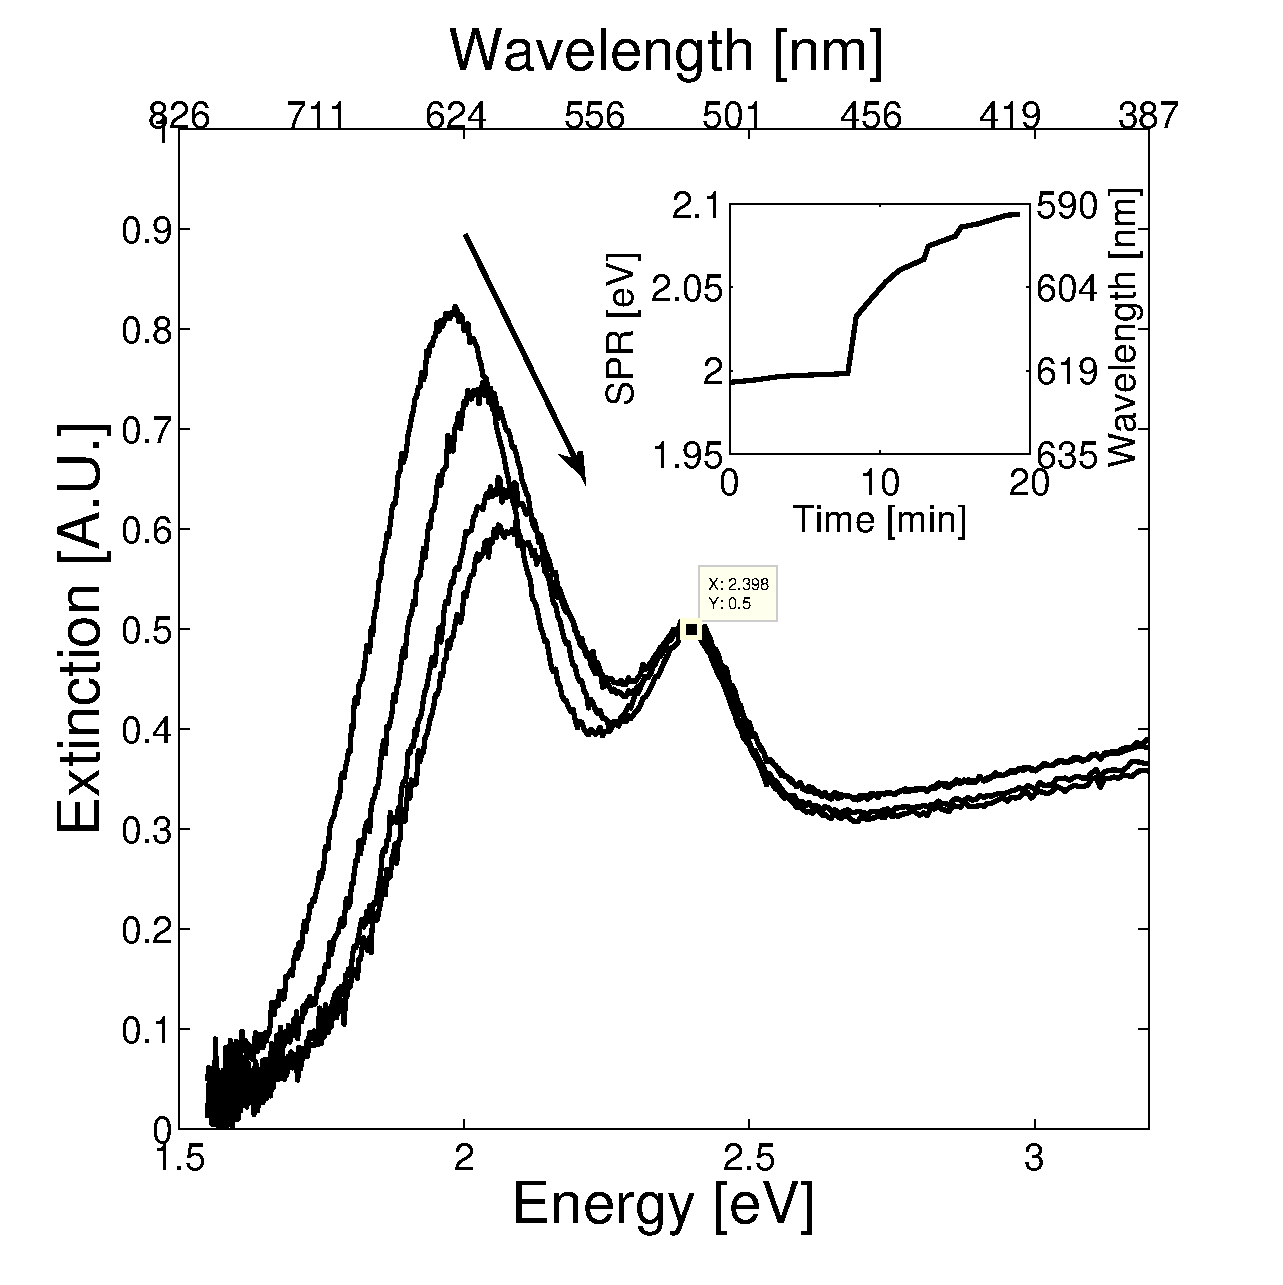
\includegraphics[width=0.95\linewidth]{plasmon_bulk.eps}
 \caption{Bulk extinction spectra at $10$ minutes time-interval. The arrow
 indicates the time evolution. A solution of KCN is added into the cuvette with
 the nanorod suspension as to have a $50\,\mu M$ concentration for the first 9
 minutes; then this step is repeated, yielding a final KCN concentration of
 $100\, \mu M$. The inset shows the peak position of the SPR position as a
 function of time, extracted by fitting the spectra with a Lorenzian.  }
 \label{fig:bulk}
\end{figure}

It can be seen that the plasmon peak position shifts towards higher energies
(from approximately $2.0\,eV$ to $2.1\,eV$ or equivantelly from $620\,nm$ to
$592\,nm$). It means that the rods are reshaping into spheres as was previously
observed\cite{janaanisotropic2002}. The asymptotic behavior of the time-trace
may be due to the small amount of KCN added into the cuvette, that reacts
entirely with gold therefore stopping the efect after a certain time.

The next set of experiments are performed in a confocal microscope for
single-particles immobilized on a glass coverslip. Figure
\ref{fig:plasmon_single_rod} shows the typical behavior of the plasmon of a
single rod while immersed in $30\,\mu M$ KCN. The Figure shows the acquired
luminescence spectra with an interval of $70\,s$ between each other; the small
shoulder at $650\,nm$ that can be observed for the less intense curves is due to
the Raman scattering of water. The inset shows the peak position (calculated by
fitting the spectra with a lorentzian) over time. It can be seen that the
plasmon red-shifts over $100\, nm$ ($0.25\, eV$) in $5$ minutes. The diminishing
intensity is consistent with the volume loss given by the dissolution of gold.
In this particular case only one rod is observed therefore having a higher
temporal resolution. However the same trend is followed by each single nanorod
analyzed under the same conditions.


\begin{figure}[hbt]
 \centering
 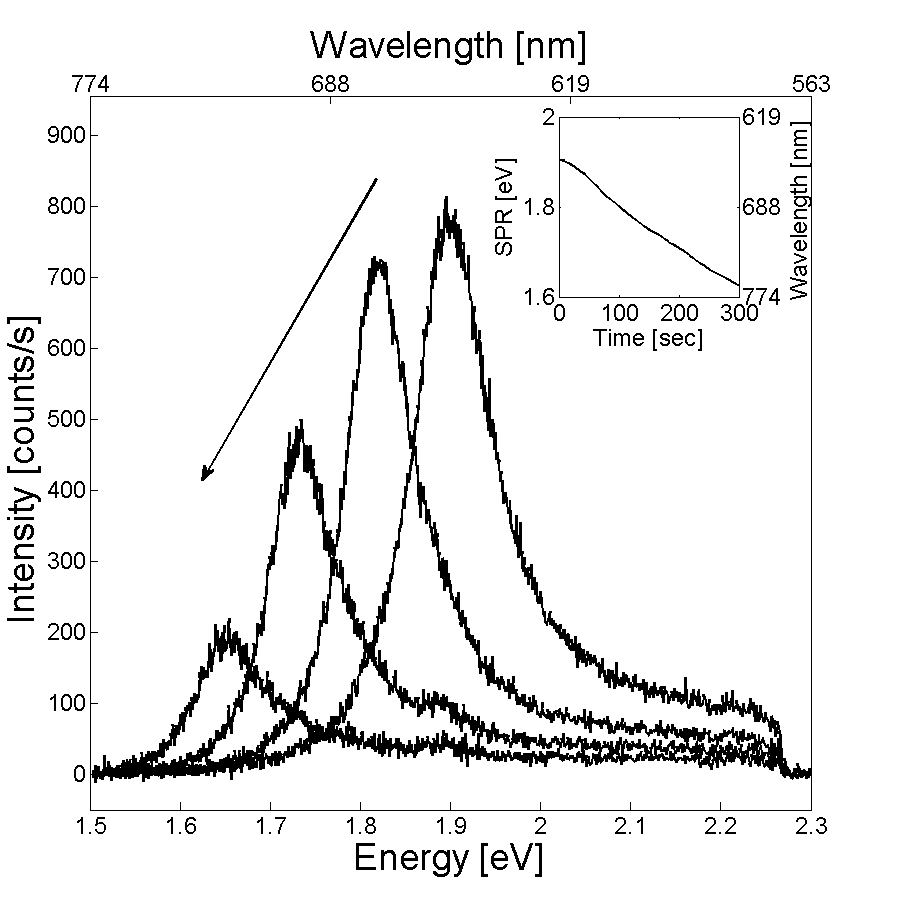
\includegraphics[width=0.95\linewidth]{plasmon_single_rod.png}
 \caption{Plasmon shift due to the etching with $30\mu M$ KCN. The time
 interval between peaks is $70s$. The inset shows the peak position of the SPR as a
 function of time, extracted by fitting the spectra with a Lorenzian.}
 \label{fig:plasmon_single_rod}
\end{figure}

These results show the opposite trend than the bulk results and therefore need a
closer study. Figure \ref{fig:plasmon_average} shows the timetraces of the peak
positions for nine different rods while being etched with $30\,\mu M$ KCN. The
pale lines show each individual trace, while the darker is the average. The error
bars are simply the standard deviation of the distribution at each point. The
bigger time step between $225\,s$ and $340\,s$ is due to an automatic refocusing
happening on the particles every $5$ minutes.

\begin{figure}[hbt]
 \centering
 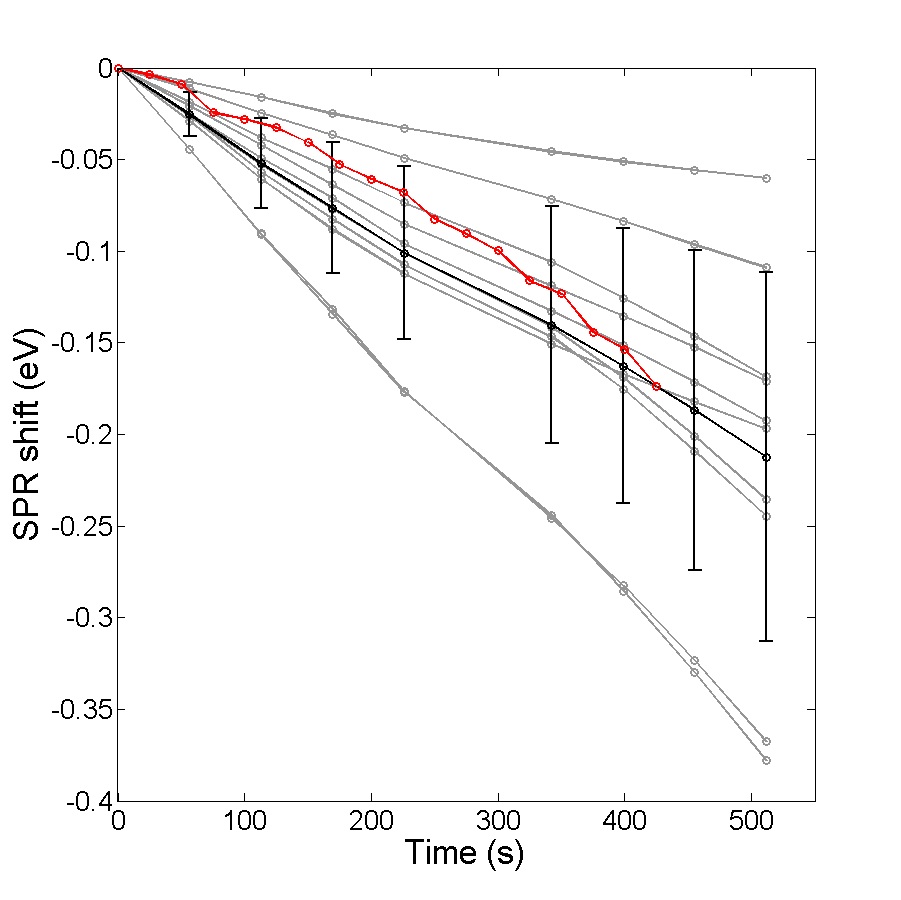
\includegraphics[width=0.95\linewidth]{plasmon_average.png}
 \caption{Average plasmon shift (thick line) for 9 rods due to the etching with
 $30\mu M$ KCN. The light curves are individual timetraces while the thick one is the
 average. The error bars are simply the standard deviation at each point. Over
 time the peak distribution gets broader.}
 \label{fig:plasmon_average}
\end{figure}

This exact same trend is observed for every particle at different KCN
concentrations. The broadening of the distribution is also observed and has to
be attributed to intrinsic inhomogenities in the particles since it is not
possible to find a trend in the shift rate nor with the initial particle 
volume nor to the initial peak position. 
% How can this be explained????

One important aspect of these results is that despite the broadening in plasmon
peak distribution over a sample the width of the plasmon peak of each individual
rod doesn't increase. Figure \ref{fig:FWHM} shows this behavior. Note that the
horizontal axis is now the peak shift and not the time. All the particles show
approximately the same behavior: narrowing of the peak up to $50\,nm$ shift and
then increasing again. The plasmon width is usally used as a quality check both
for knowing that they are single particles and for possible changes in shape.

\begin{figure}[hbt]
 \centering
 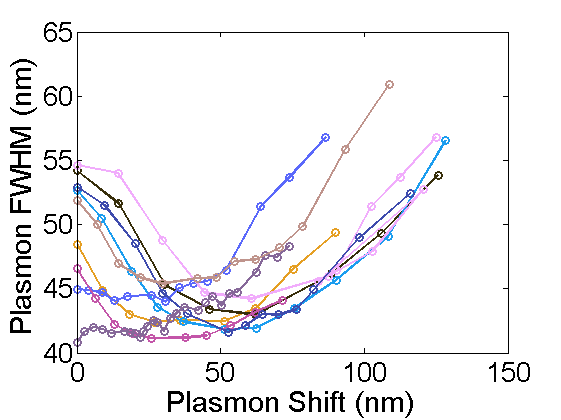
\includegraphics[width=0.95\linewidth]{fwhm_several.png}
 \caption{Plasmon FWHM of nine different particles immersed in $30\,\mu M$ KCN
 as a function of their plasmon shift.}
 \label{fig:FWHM}
\end{figure}

For understanding these results a simple model of isotropic etching may be
considered. It is assumed that the nanorods diminish their length and radius at
the same rate. The extinction cross section spectra is then calculated for
several time steps using the ADDA package. The peaks are extracted from the
simulations in the same way than for the experiments. The results are displayed
as the red curve in Figure \ref{fig:plasmon_average}. The best approximation to
the average is found when the etching rate is set to $1\,nm/min$.

Figure \ref{fig:SEM_30muM} shows three SEM images for a sample of the same
nanorods used in the optical experiment before the etching, after $2min$
submersed in KCN and after $4min$. The histograms show the distribution of
aspect ratios at the three given instants. Table \ref{tab:SEM_results}
summarizes the averaged values found after analyzing approximately $300$
particles. It is possible to observe that the AuNR preserve the shape while
diminishing the volume and increasing the aspect ratio. Nevertheless this
changes are inside the standard distribution of each parameter. However the
small shift in the average is consistent with the optical results, yielding an
etching rate of $0.5\,nm\min$.

\begin{tabular*}{0.48\textwidth}{c c c c c}
 $\,$ & L (nm) & Sdv (nm) & R (nm) & Sdv (nm) \\\hline
 $0min$ & $51$ & $5$ & $24$ & $3$ \\ 
 $2min$ & $50$ & $5$ & $23$ & $3$ \\
 $4min$ & $49$ & $5$ & $22$ & $2$ \\
\label{tab:SEM_results}

\end{tabular*}


\section{Conclusions}
In this work it is shown a simple method that allows the tuning of the plasmon
peak position of a single gold nanorod with nanometer accuracy. More
importantly, it is shown that the rodlike shape is preserved even for plasmon
shifts of approximately $80nm$ therefore keeping the well known properties of
them.

The optical experiments show the red-shift of the plasmon with a high time
accuracy, while with the SEM it is possible to confirm that the shape of the
rods is being preserved. The agreement between the simulations and the
experimental results not only show the link between both measurments but also
provide a way of predicting the behaviour of the plasmon peak. 

However, it is also found a great distribution width at the rate plasmon shifts
for different particles under the same experimental conditions. This can be
explained only considering that there is an intrinsic difference between
particles; this differences can be attributed to defects on the particle surface
or to inhomogenities in the CTAB present; even if care is taken to remove it
by rinsing with water it may be that some remains sticked to the particle.

Combining this results with the catalytic properties of gold and the presence of
the plasmon resonance opens the door for fine-controlling chemical reactions
while irradiating the particles with specific wavelengths.

\bibliography{bibliography}{}
\bibliographystyle{plain}

\end{document}
